\documentclass[11pt]{article}
\usepackage[textwidth=18.0cm, textheight=23.0cm, top=2.0cm]{geometry}
\usepackage{pst-all}
\usepackage{amssymb}
\usepackage{tikz}
\usepackage{underscore}\begin{document}
\pagestyle{empty}


ClassName: \underline{\textbf{Class_05.2bp-19}}
\par
BinSize: \underline{\textbf{100 × 100}}
\par
ReduceSize: \underline{\textbf{100 × 100}}
\par
TypeNum: \underline{\textbf{40}}
\par
Num: \underline{\textbf{40}}
\par
OutS: \underline{\textbf{100000}}
\par
InS: \underline{\textbf{84528}}
\par
Rate: \underline{\textbf{0.845}}
\par
UB: \underline{\textbf{10}}
\par
LB0: \underline{\textbf{10}}
\par
LB: \underline{\textbf{10}}
\par
LBWithCut: \underline{\textbf{10}}
\par
NodeCut: \underline{\textbf{0}}
\par
ExtendedNodeCnt: \underline{\textbf{1}}
\par
GenNodeCnt: \underline{\textbf{1}}
\par
PrimalNode: \underline{\textbf{0}}
\par
ColumnCount: \underline{\textbf{10}}
\par
TotalCutCount: \underline{\textbf{0}}
\par
RootCutCount: \underline{\textbf{0}}
\par
LPSolverCnt: \underline{\textbf{1}}
\par
PricingSolverCnt: \underline{\textbf{0}}
\par
BranchAndBoundNum: \underline{\textbf{1}}
\par
isOpt: \underline{\textbf{true}}
\par
TimeOnInitSolution: \underline{\textbf{0.060 s}}
\par
TimeOnPrimal: \underline{\textbf{0.000 s}}
\par
TimeOnPricing: \underline{\textbf{0.000 s}}
\par
TimeOnRmp: \underline{\textbf{0.083 s}}
\par
TotalTime: \underline{\textbf{0.210 s}}
\par
\newpage


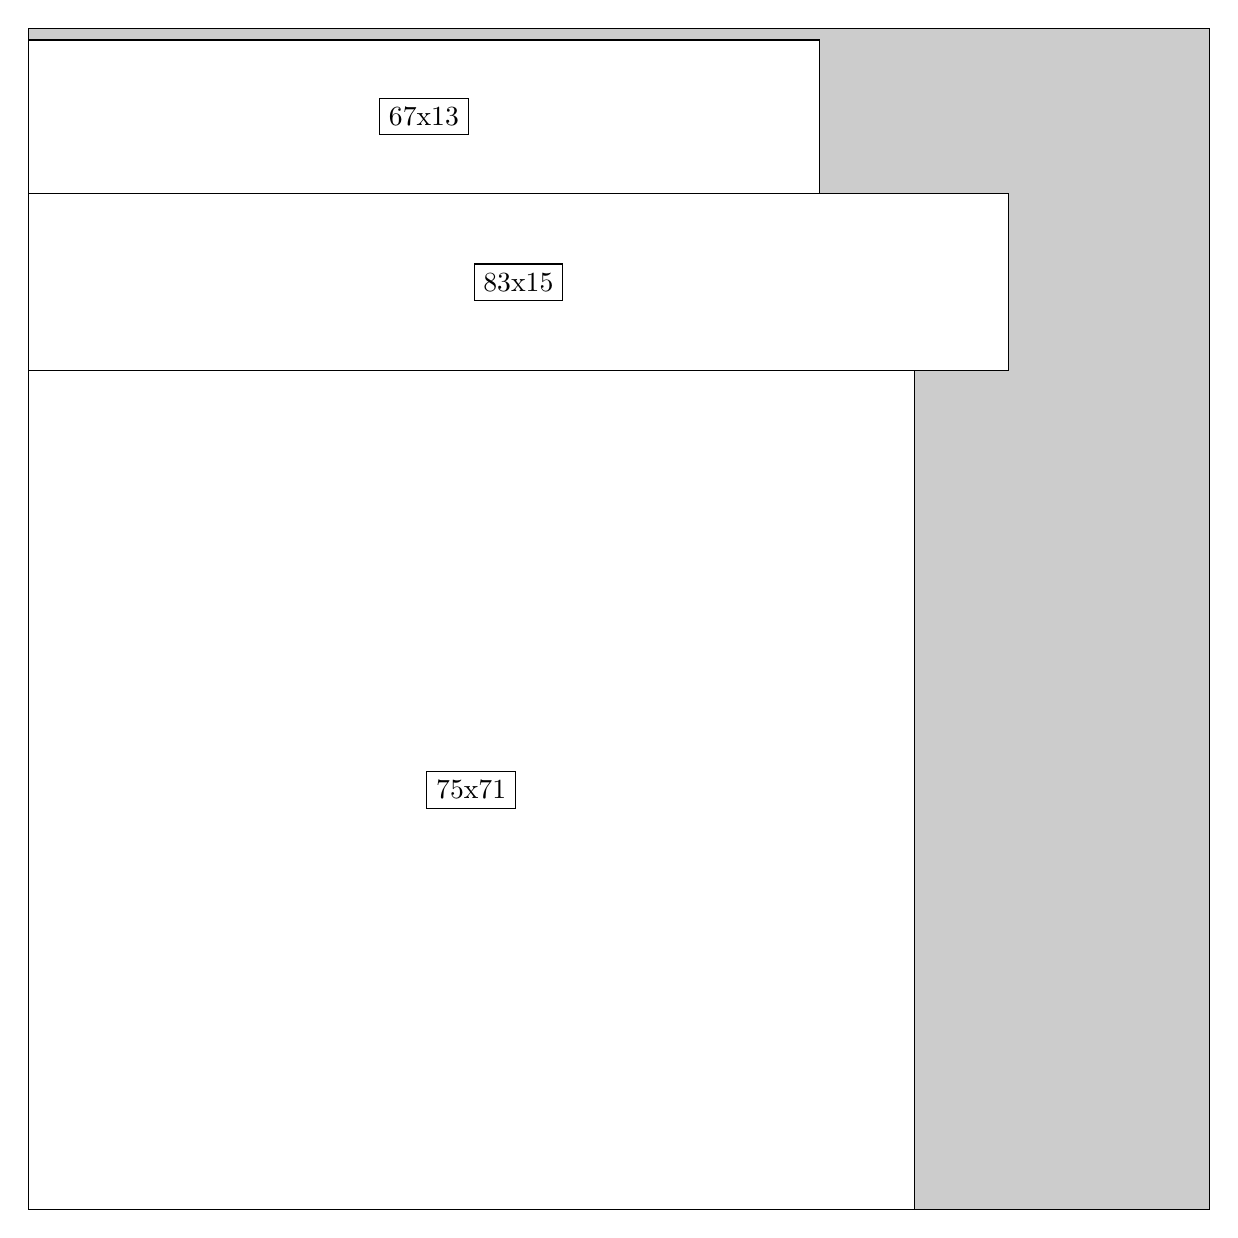
\begin{tikzpicture}[shorten >=1pt,scale=1.0,every node/.style={scale=1.0},->]
\tikzstyle{vertex}=[circle,fill=black!25,minimum size=14pt,inner sep=0pt]
\filldraw[fill=gray!40!white, draw=black] (0,0) rectangle (15.0,15.0);
\foreach \name/\x/\y/\w/\h in {75x71/0.0/0.0/11.25/10.65,83x15/0.0/10.65/12.45/2.25,67x13/0.0/12.9/10.049999999999999/1.95}
\filldraw[fill=white!40!white, draw=black] (\x,\y) rectangle node[draw] (\name) {\name} ++(\w,\h);
\end{tikzpicture}


w =75 , h =71 , x =0 , y =0 , v =5325
\par
w =83 , h =15 , x =0 , y =71 , v =1245
\par
w =67 , h =13 , x =0 , y =86 , v =871
\par
\newpage


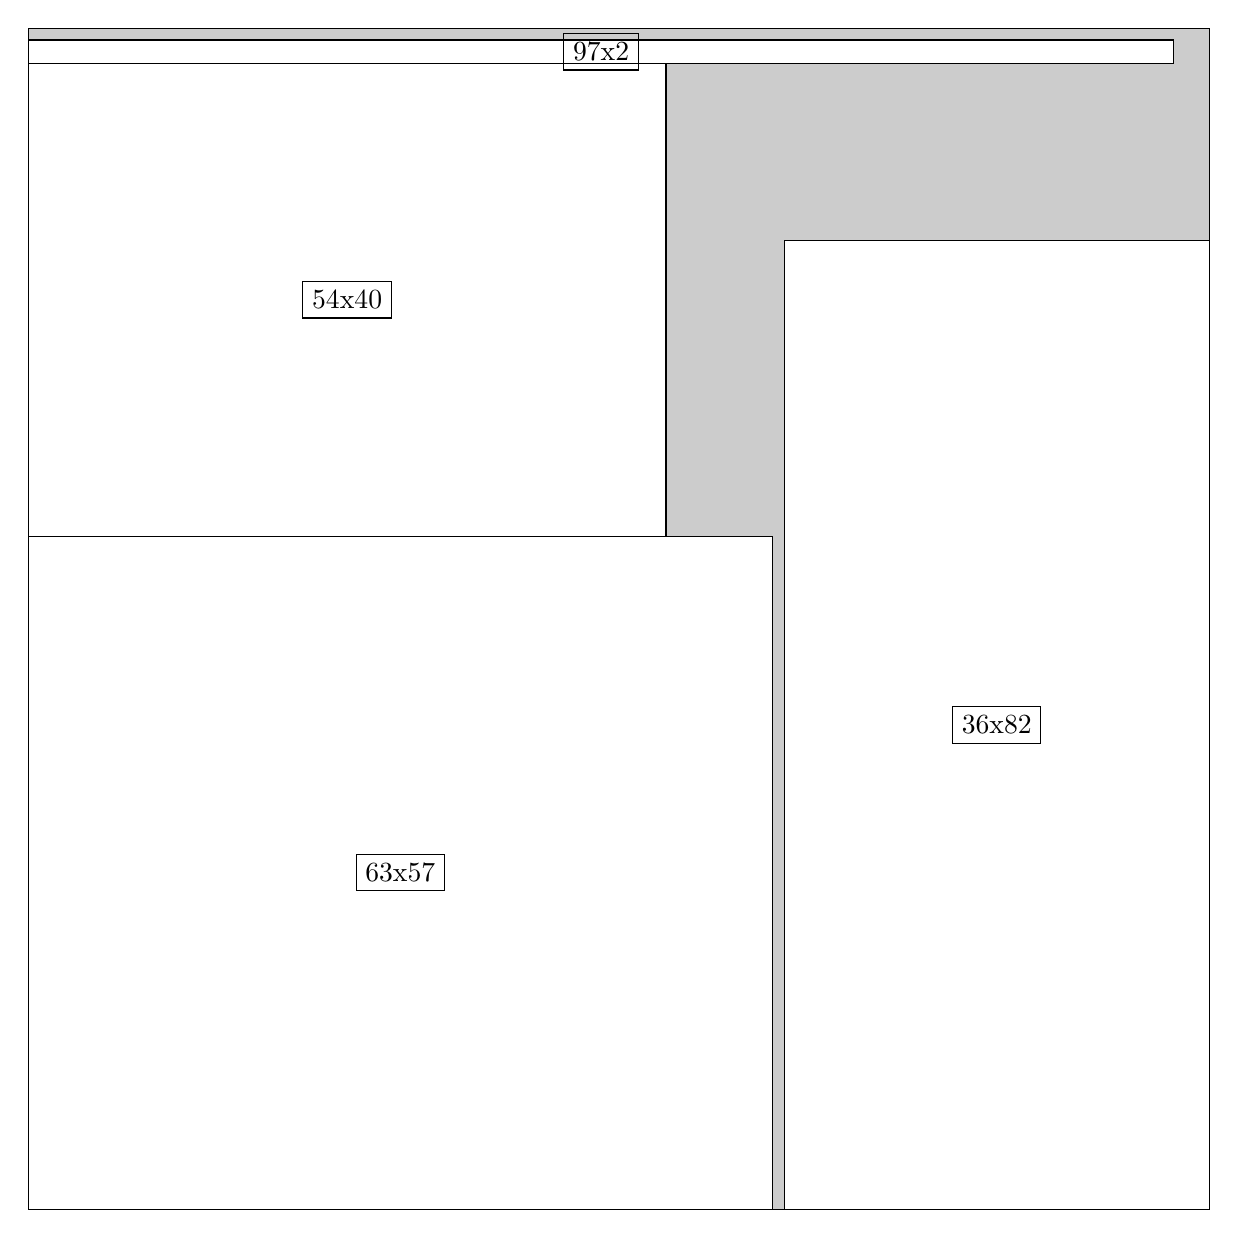
\begin{tikzpicture}[shorten >=1pt,scale=1.0,every node/.style={scale=1.0},->]
\tikzstyle{vertex}=[circle,fill=black!25,minimum size=14pt,inner sep=0pt]
\filldraw[fill=gray!40!white, draw=black] (0,0) rectangle (15.0,15.0);
\foreach \name/\x/\y/\w/\h in {63x57/0.0/0.0/9.45/8.549999999999999,54x40/0.0/8.549999999999999/8.1/6.0,36x82/9.6/0.0/5.3999999999999995/12.299999999999999,97x2/0.0/14.549999999999999/14.549999999999999/0.3}
\filldraw[fill=white!40!white, draw=black] (\x,\y) rectangle node[draw] (\name) {\name} ++(\w,\h);
\end{tikzpicture}


w =63 , h =57 , x =0 , y =0 , v =3591
\par
w =54 , h =40 , x =0 , y =57 , v =2160
\par
w =36 , h =82 , x =64 , y =0 , v =2952
\par
w =97 , h =2 , x =0 , y =97 , v =194
\par
\newpage


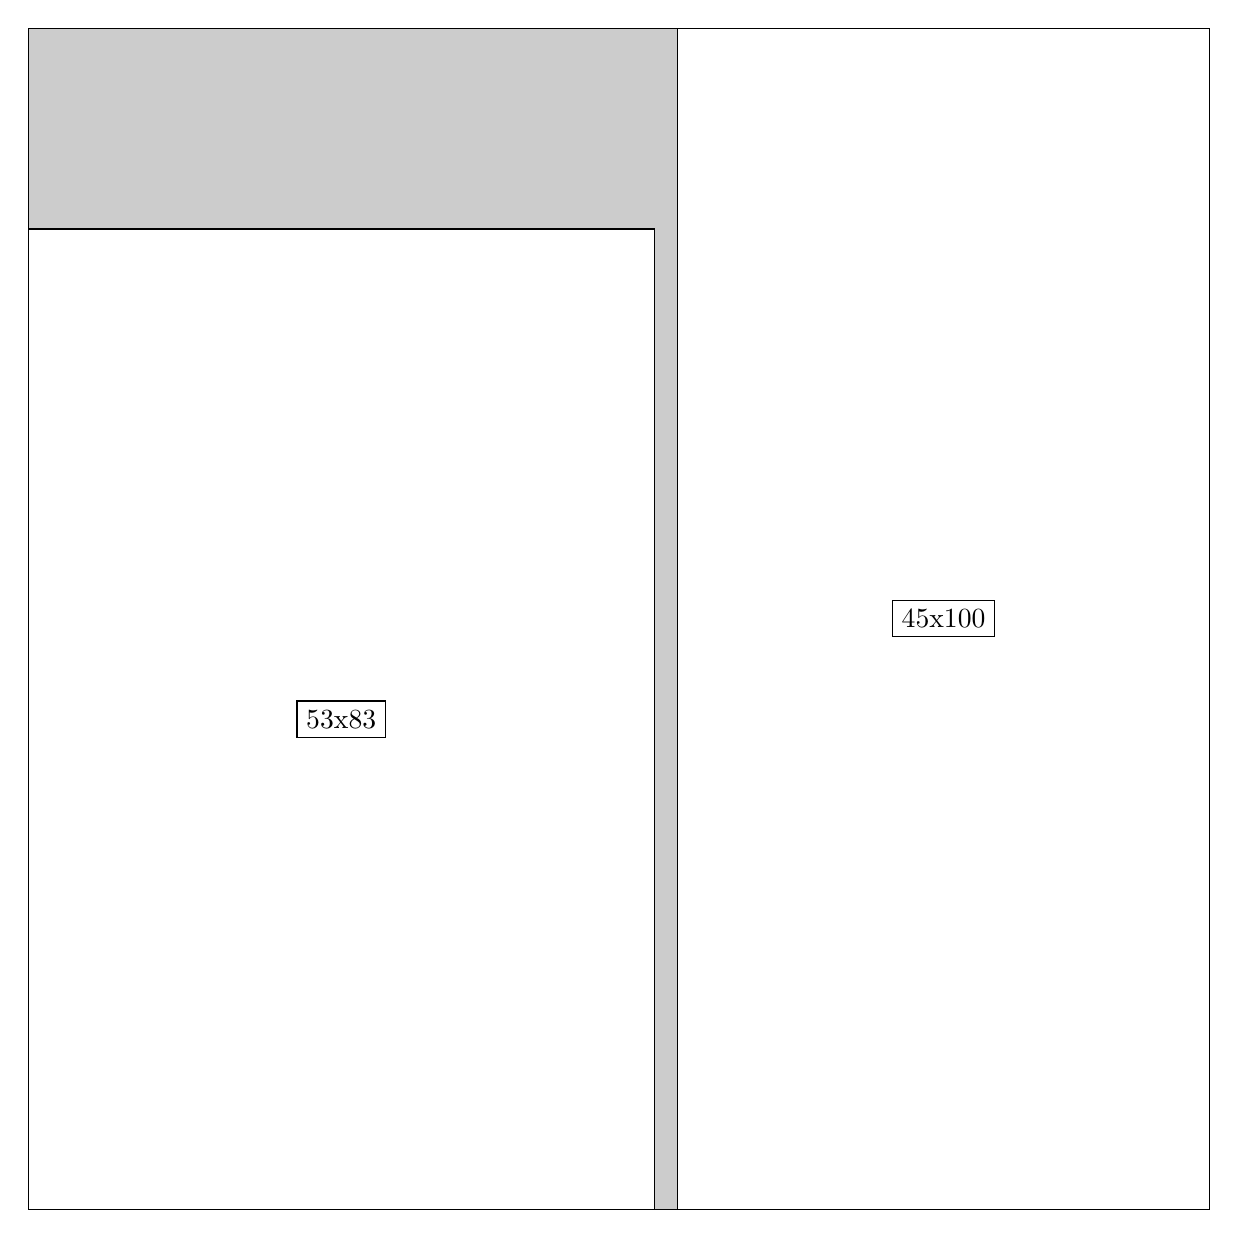
\begin{tikzpicture}[shorten >=1pt,scale=1.0,every node/.style={scale=1.0},->]
\tikzstyle{vertex}=[circle,fill=black!25,minimum size=14pt,inner sep=0pt]
\filldraw[fill=gray!40!white, draw=black] (0,0) rectangle (15.0,15.0);
\foreach \name/\x/\y/\w/\h in {45x100/8.25/0.0/6.75/15.0,53x83/0.0/0.0/7.949999999999999/12.45}
\filldraw[fill=white!40!white, draw=black] (\x,\y) rectangle node[draw] (\name) {\name} ++(\w,\h);
\end{tikzpicture}


w =45 , h =100 , x =55 , y =0 , v =4500
\par
w =53 , h =83 , x =0 , y =0 , v =4399
\par
\newpage


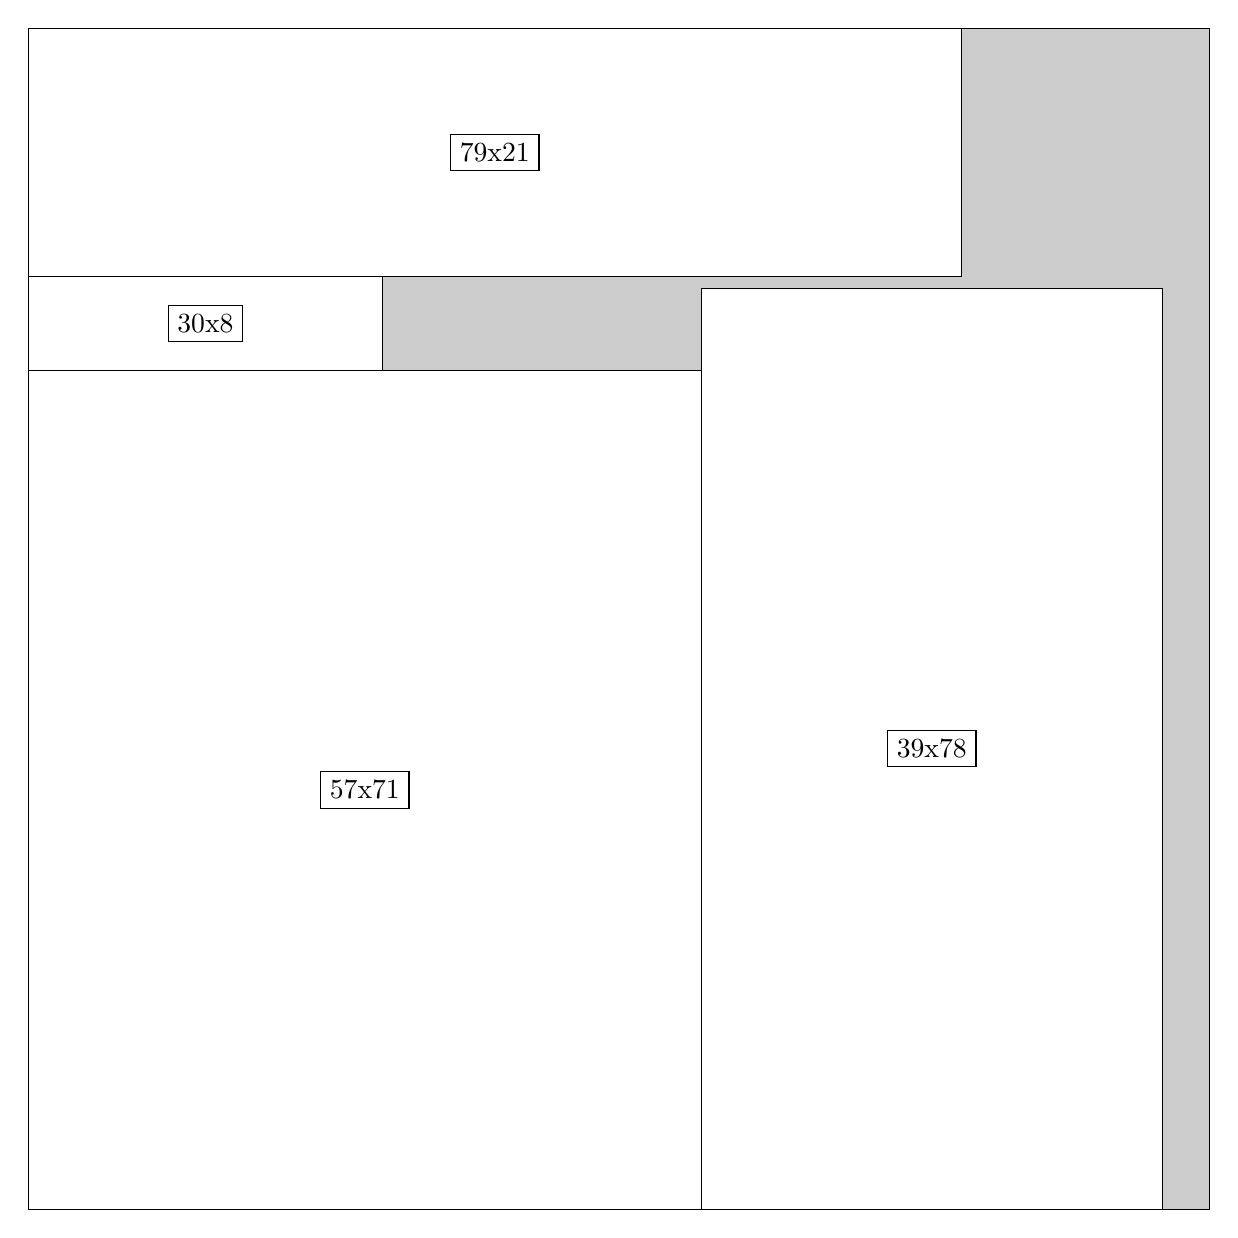
\begin{tikzpicture}[shorten >=1pt,scale=1.0,every node/.style={scale=1.0},->]
\tikzstyle{vertex}=[circle,fill=black!25,minimum size=14pt,inner sep=0pt]
\filldraw[fill=gray!40!white, draw=black] (0,0) rectangle (15.0,15.0);
\foreach \name/\x/\y/\w/\h in {57x71/0.0/0.0/8.549999999999999/10.65,39x78/8.549999999999999/0.0/5.85/11.7,30x8/0.0/10.65/4.5/1.2,79x21/0.0/11.85/11.85/3.15}
\filldraw[fill=white!40!white, draw=black] (\x,\y) rectangle node[draw] (\name) {\name} ++(\w,\h);
\end{tikzpicture}


w =57 , h =71 , x =0 , y =0 , v =4047
\par
w =39 , h =78 , x =57 , y =0 , v =3042
\par
w =30 , h =8 , x =0 , y =71 , v =240
\par
w =79 , h =21 , x =0 , y =79 , v =1659
\par
\newpage


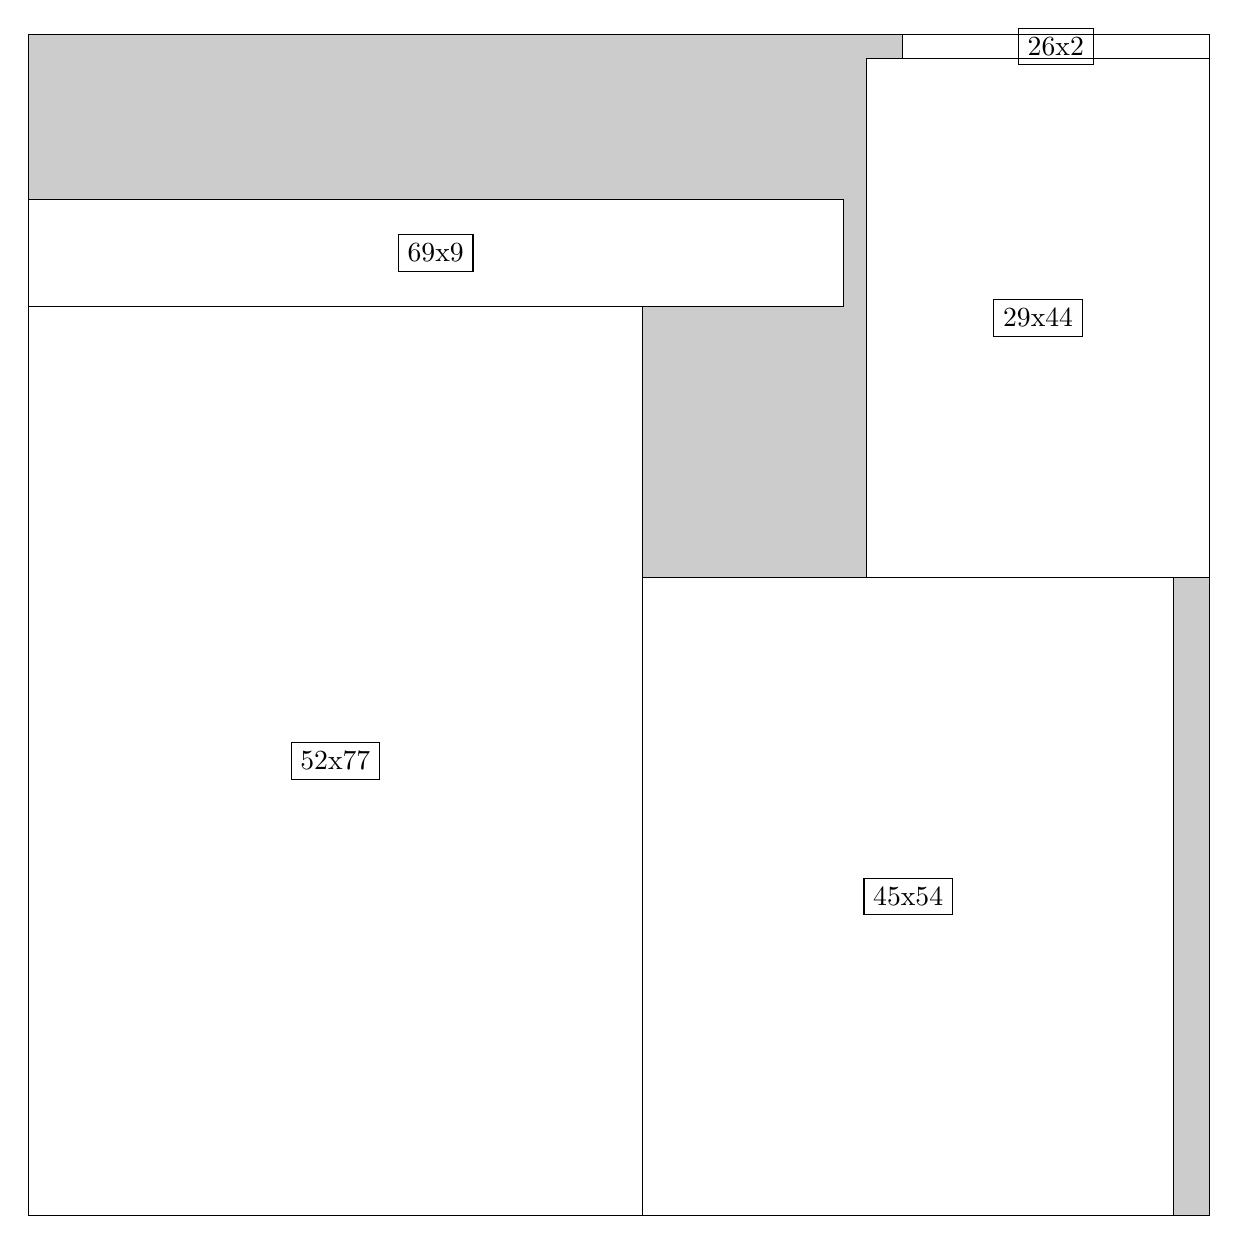
\begin{tikzpicture}[shorten >=1pt,scale=1.0,every node/.style={scale=1.0},->]
\tikzstyle{vertex}=[circle,fill=black!25,minimum size=14pt,inner sep=0pt]
\filldraw[fill=gray!40!white, draw=black] (0,0) rectangle (15.0,15.0);
\foreach \name/\x/\y/\w/\h in {52x77/0.0/0.0/7.8/11.549999999999999,45x54/7.8/0.0/6.75/8.1,29x44/10.65/8.1/4.35/6.6,69x9/0.0/11.549999999999999/10.35/1.3499999999999999,26x2/11.1/14.7/3.9/0.3}
\filldraw[fill=white!40!white, draw=black] (\x,\y) rectangle node[draw] (\name) {\name} ++(\w,\h);
\end{tikzpicture}


w =52 , h =77 , x =0 , y =0 , v =4004
\par
w =45 , h =54 , x =52 , y =0 , v =2430
\par
w =29 , h =44 , x =71 , y =54 , v =1276
\par
w =69 , h =9 , x =0 , y =77 , v =621
\par
w =26 , h =2 , x =74 , y =98 , v =52
\par
\newpage


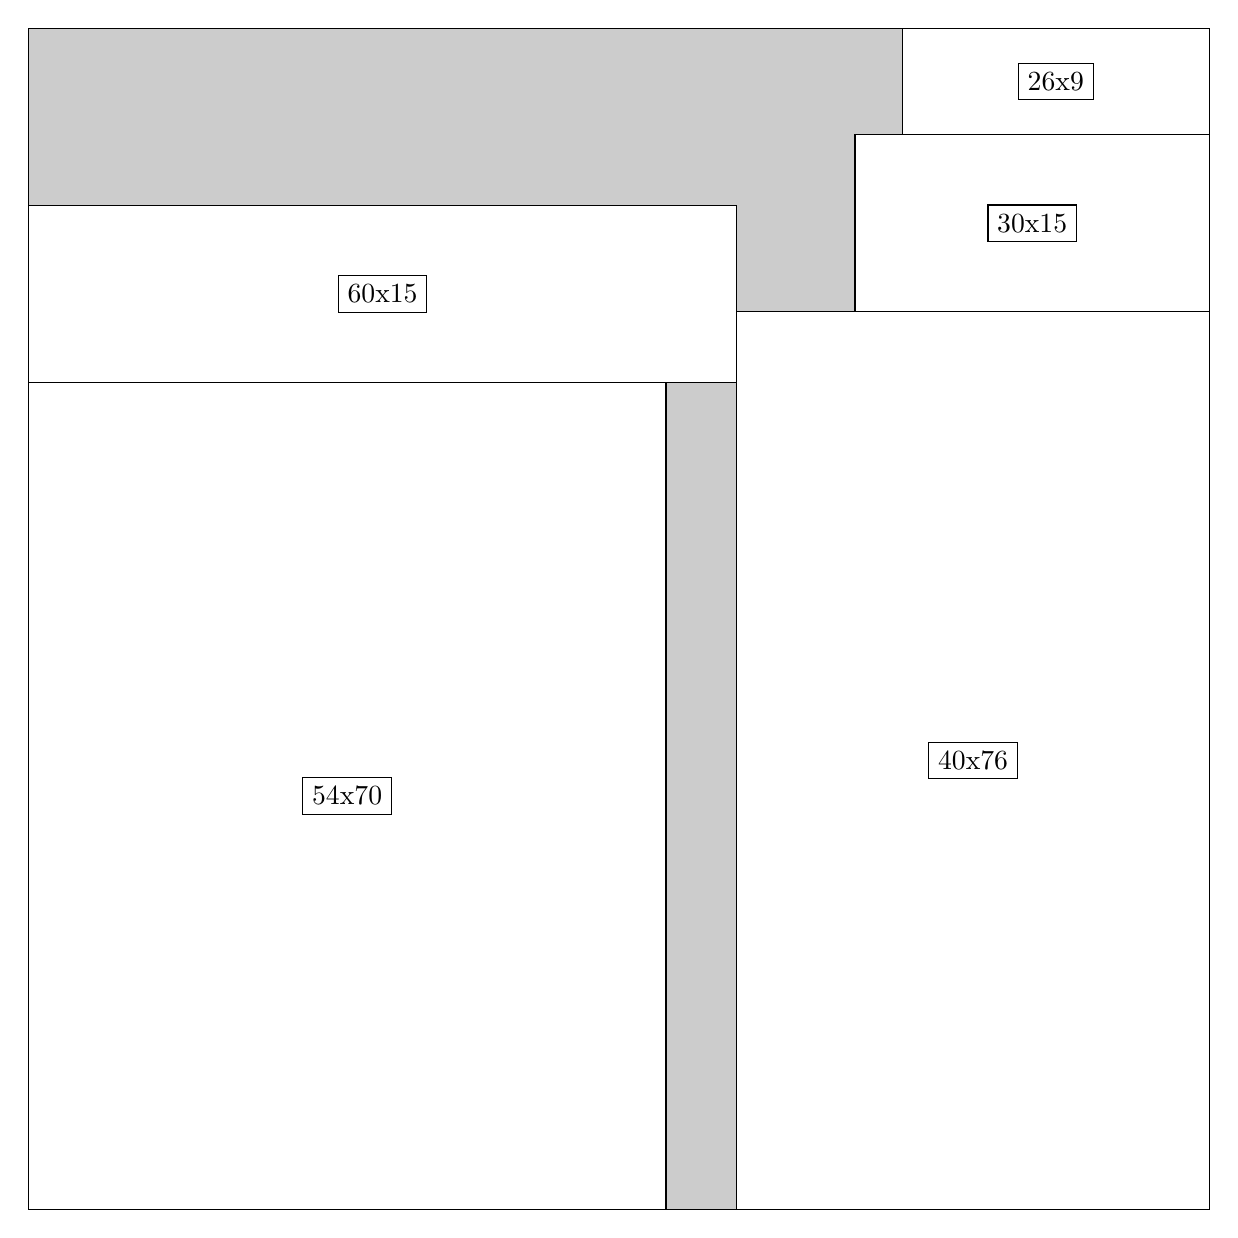
\begin{tikzpicture}[shorten >=1pt,scale=1.0,every node/.style={scale=1.0},->]
\tikzstyle{vertex}=[circle,fill=black!25,minimum size=14pt,inner sep=0pt]
\filldraw[fill=gray!40!white, draw=black] (0,0) rectangle (15.0,15.0);
\foreach \name/\x/\y/\w/\h in {54x70/0.0/0.0/8.1/10.5,40x76/9.0/0.0/6.0/11.4,60x15/0.0/10.5/9.0/2.25,30x15/10.5/11.4/4.5/2.25,26x9/11.1/13.65/3.9/1.3499999999999999}
\filldraw[fill=white!40!white, draw=black] (\x,\y) rectangle node[draw] (\name) {\name} ++(\w,\h);
\end{tikzpicture}


w =54 , h =70 , x =0 , y =0 , v =3780
\par
w =40 , h =76 , x =60 , y =0 , v =3040
\par
w =60 , h =15 , x =0 , y =70 , v =900
\par
w =30 , h =15 , x =70 , y =76 , v =450
\par
w =26 , h =9 , x =74 , y =91 , v =234
\par
\newpage


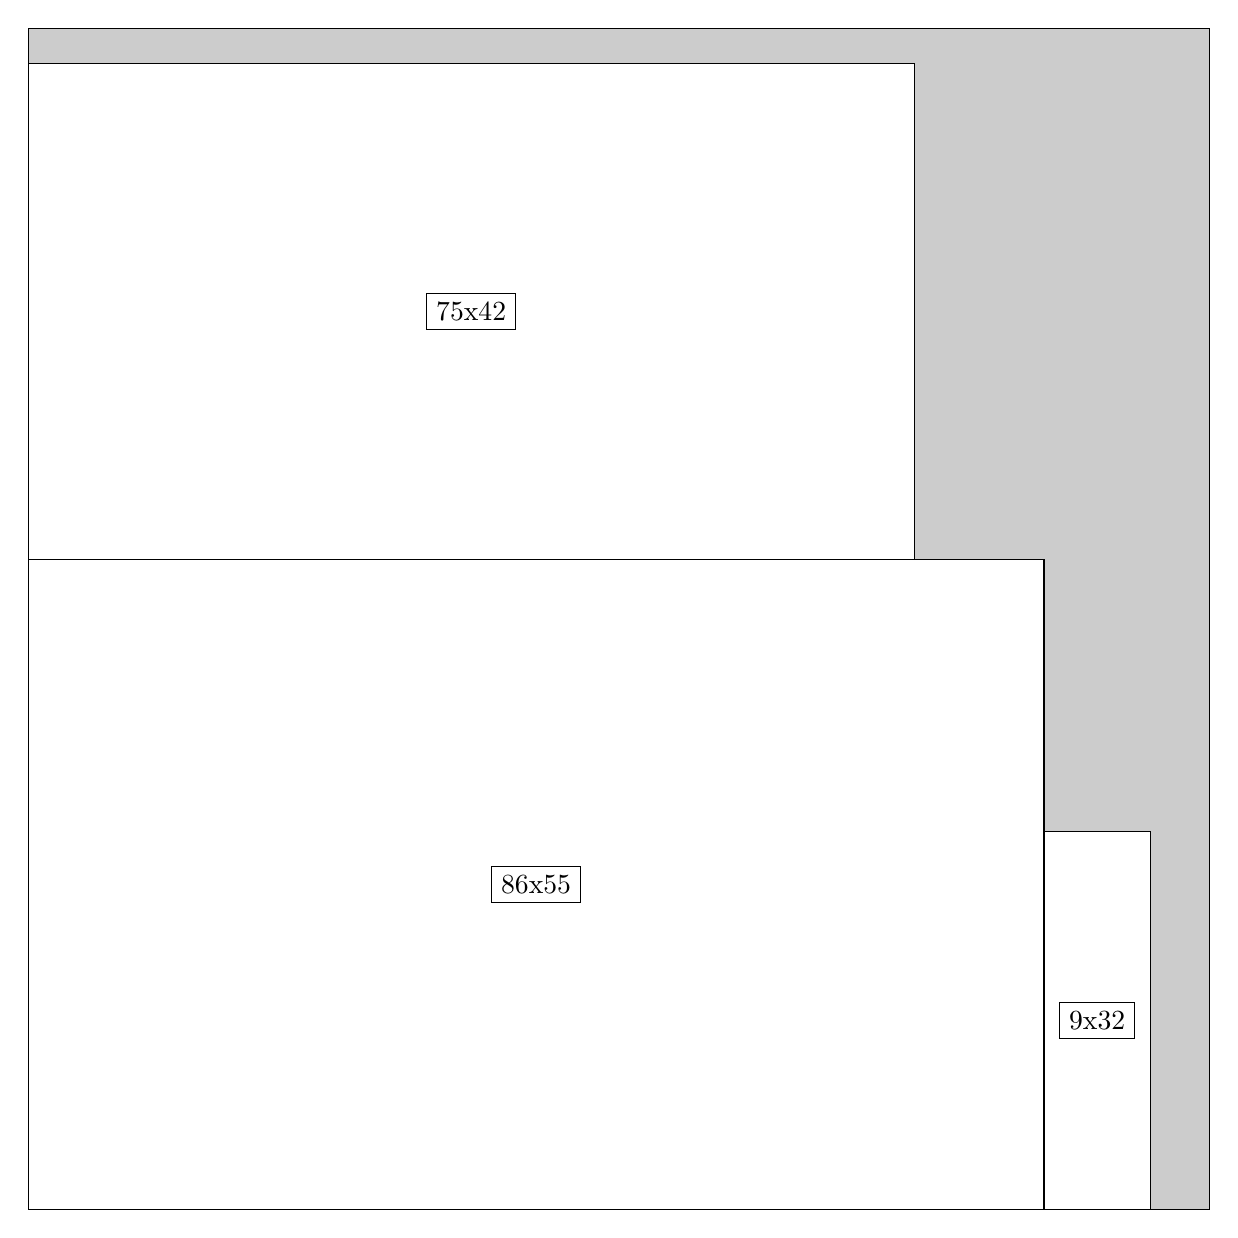
\begin{tikzpicture}[shorten >=1pt,scale=1.0,every node/.style={scale=1.0},->]
\tikzstyle{vertex}=[circle,fill=black!25,minimum size=14pt,inner sep=0pt]
\filldraw[fill=gray!40!white, draw=black] (0,0) rectangle (15.0,15.0);
\foreach \name/\x/\y/\w/\h in {75x42/0.0/8.25/11.25/6.3,86x55/0.0/0.0/12.9/8.25,9x32/12.9/0.0/1.3499999999999999/4.8}
\filldraw[fill=white!40!white, draw=black] (\x,\y) rectangle node[draw] (\name) {\name} ++(\w,\h);
\end{tikzpicture}


w =75 , h =42 , x =0 , y =55 , v =3150
\par
w =86 , h =55 , x =0 , y =0 , v =4730
\par
w =9 , h =32 , x =86 , y =0 , v =288
\par
\newpage


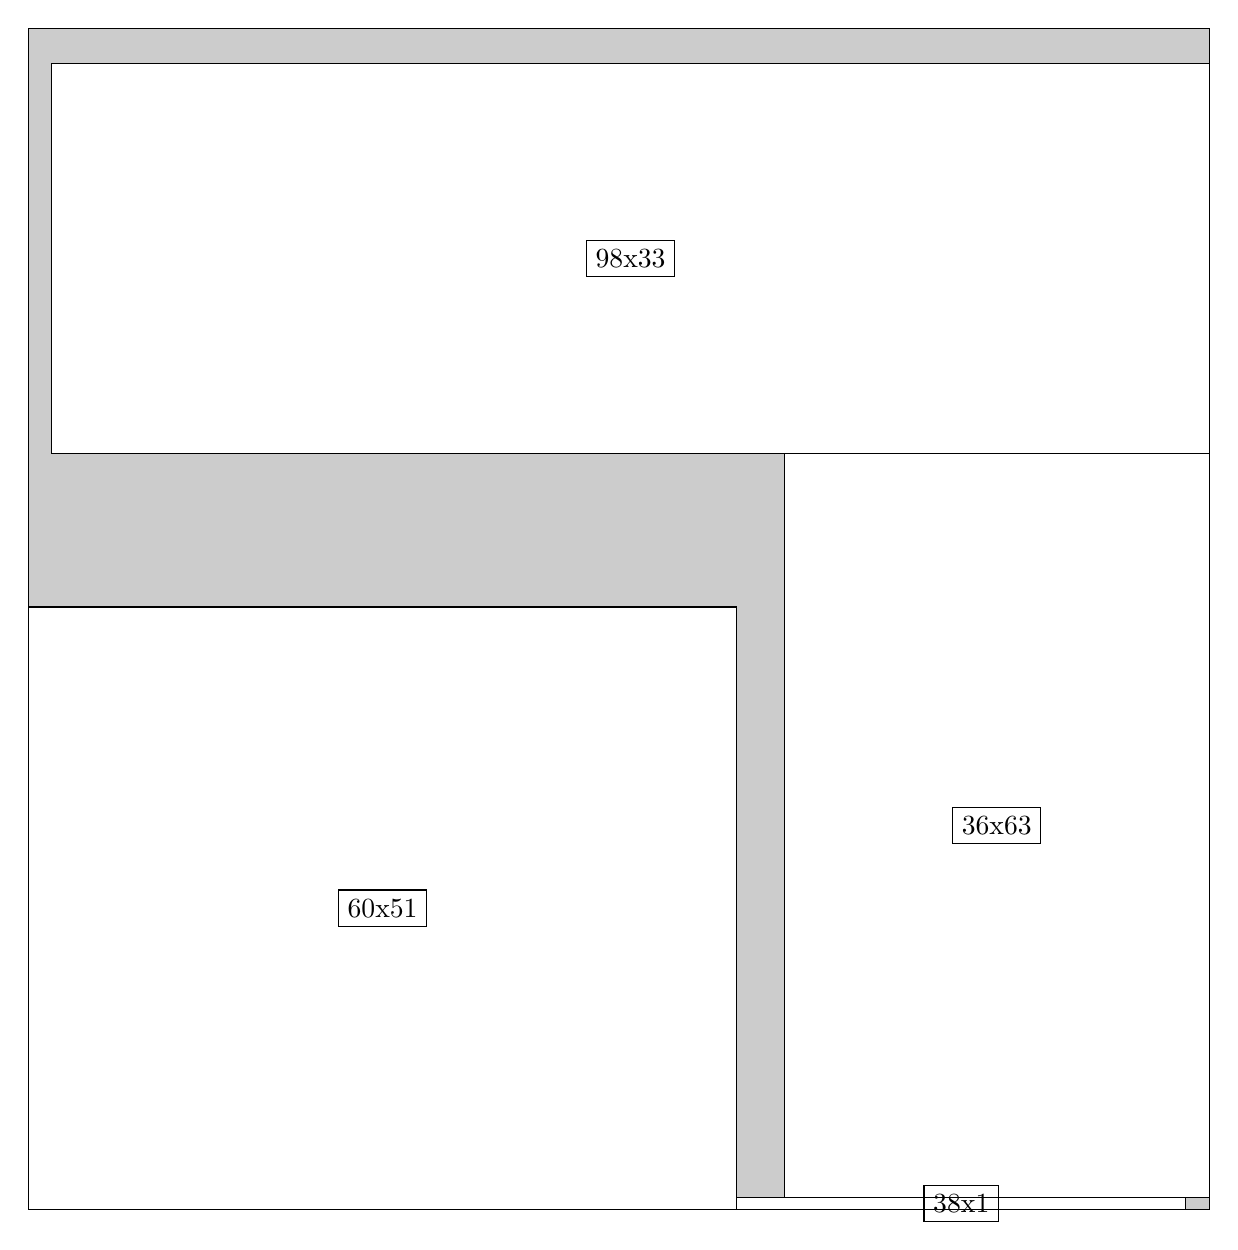
\begin{tikzpicture}[shorten >=1pt,scale=1.0,every node/.style={scale=1.0},->]
\tikzstyle{vertex}=[circle,fill=black!25,minimum size=14pt,inner sep=0pt]
\filldraw[fill=gray!40!white, draw=black] (0,0) rectangle (15.0,15.0);
\foreach \name/\x/\y/\w/\h in {98x33/0.3/9.6/14.7/4.95,60x51/0.0/0.0/9.0/7.6499999999999995,36x63/9.6/0.15/5.3999999999999995/9.45,38x1/9.0/0.0/5.7/0.15}
\filldraw[fill=white!40!white, draw=black] (\x,\y) rectangle node[draw] (\name) {\name} ++(\w,\h);
\end{tikzpicture}


w =98 , h =33 , x =2 , y =64 , v =3234
\par
w =60 , h =51 , x =0 , y =0 , v =3060
\par
w =36 , h =63 , x =64 , y =1 , v =2268
\par
w =38 , h =1 , x =60 , y =0 , v =38
\par
\newpage


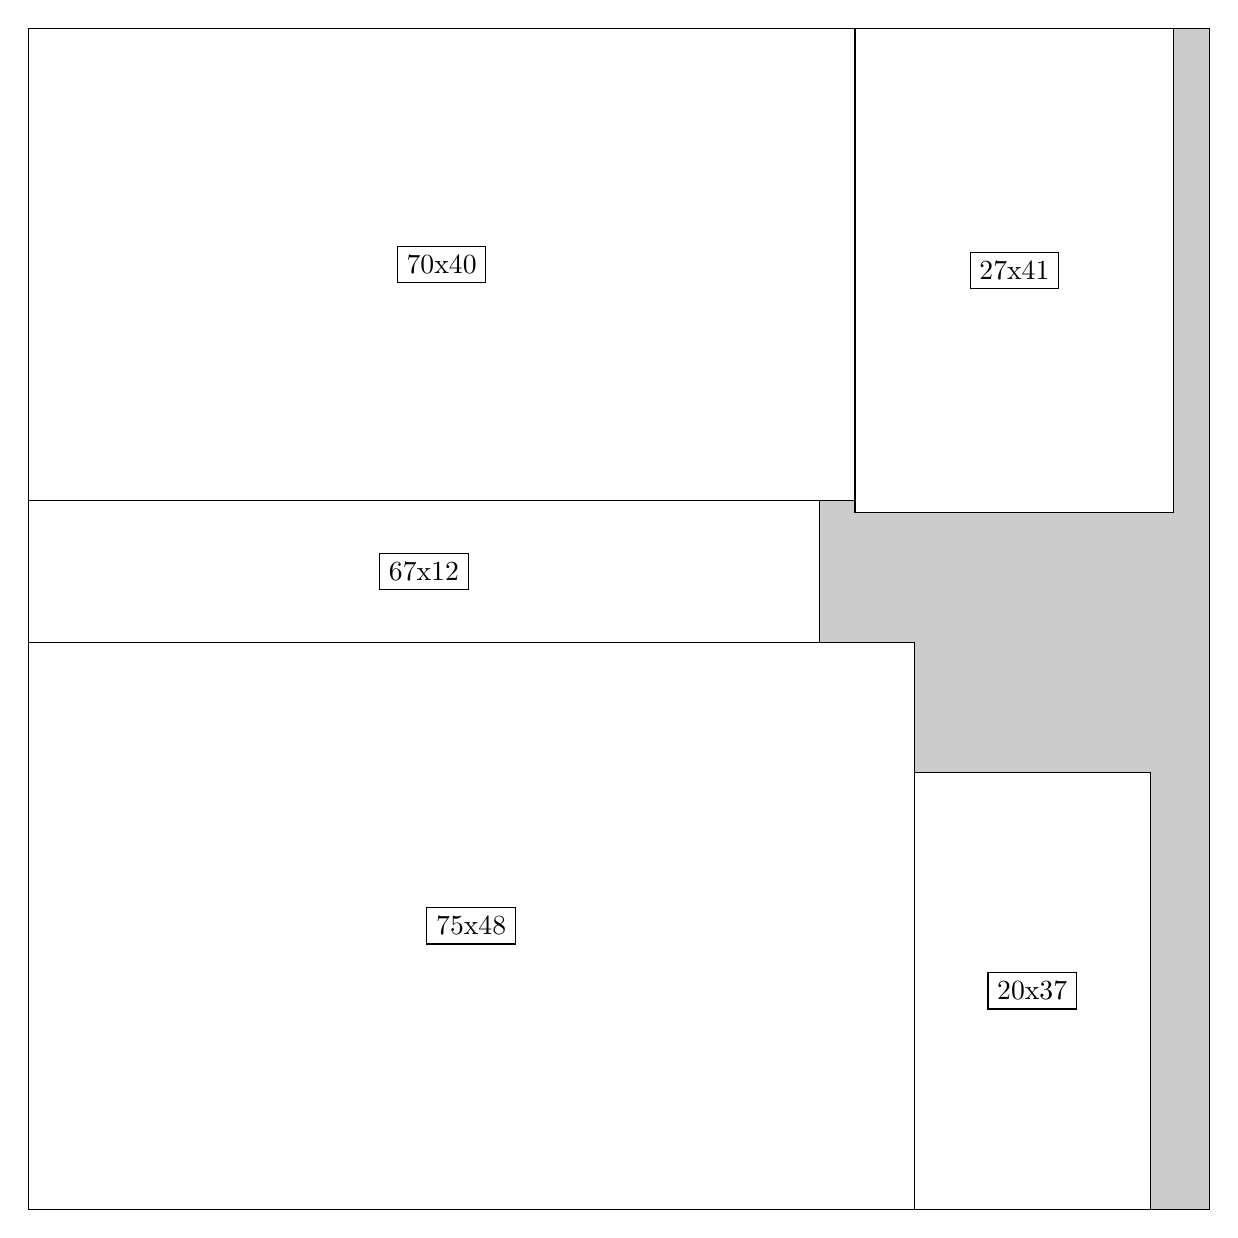
\begin{tikzpicture}[shorten >=1pt,scale=1.0,every node/.style={scale=1.0},->]
\tikzstyle{vertex}=[circle,fill=black!25,minimum size=14pt,inner sep=0pt]
\filldraw[fill=gray!40!white, draw=black] (0,0) rectangle (15.0,15.0);
\foreach \name/\x/\y/\w/\h in {75x48/0.0/0.0/11.25/7.199999999999999,27x41/10.5/8.85/4.05/6.1499999999999995,67x12/0.0/7.199999999999999/10.049999999999999/1.7999999999999998,20x37/11.25/0.0/3.0/5.55,70x40/0.0/9.0/10.5/6.0}
\filldraw[fill=white!40!white, draw=black] (\x,\y) rectangle node[draw] (\name) {\name} ++(\w,\h);
\end{tikzpicture}


w =75 , h =48 , x =0 , y =0 , v =3600
\par
w =27 , h =41 , x =70 , y =59 , v =1107
\par
w =67 , h =12 , x =0 , y =48 , v =804
\par
w =20 , h =37 , x =75 , y =0 , v =740
\par
w =70 , h =40 , x =0 , y =60 , v =2800
\par
\newpage


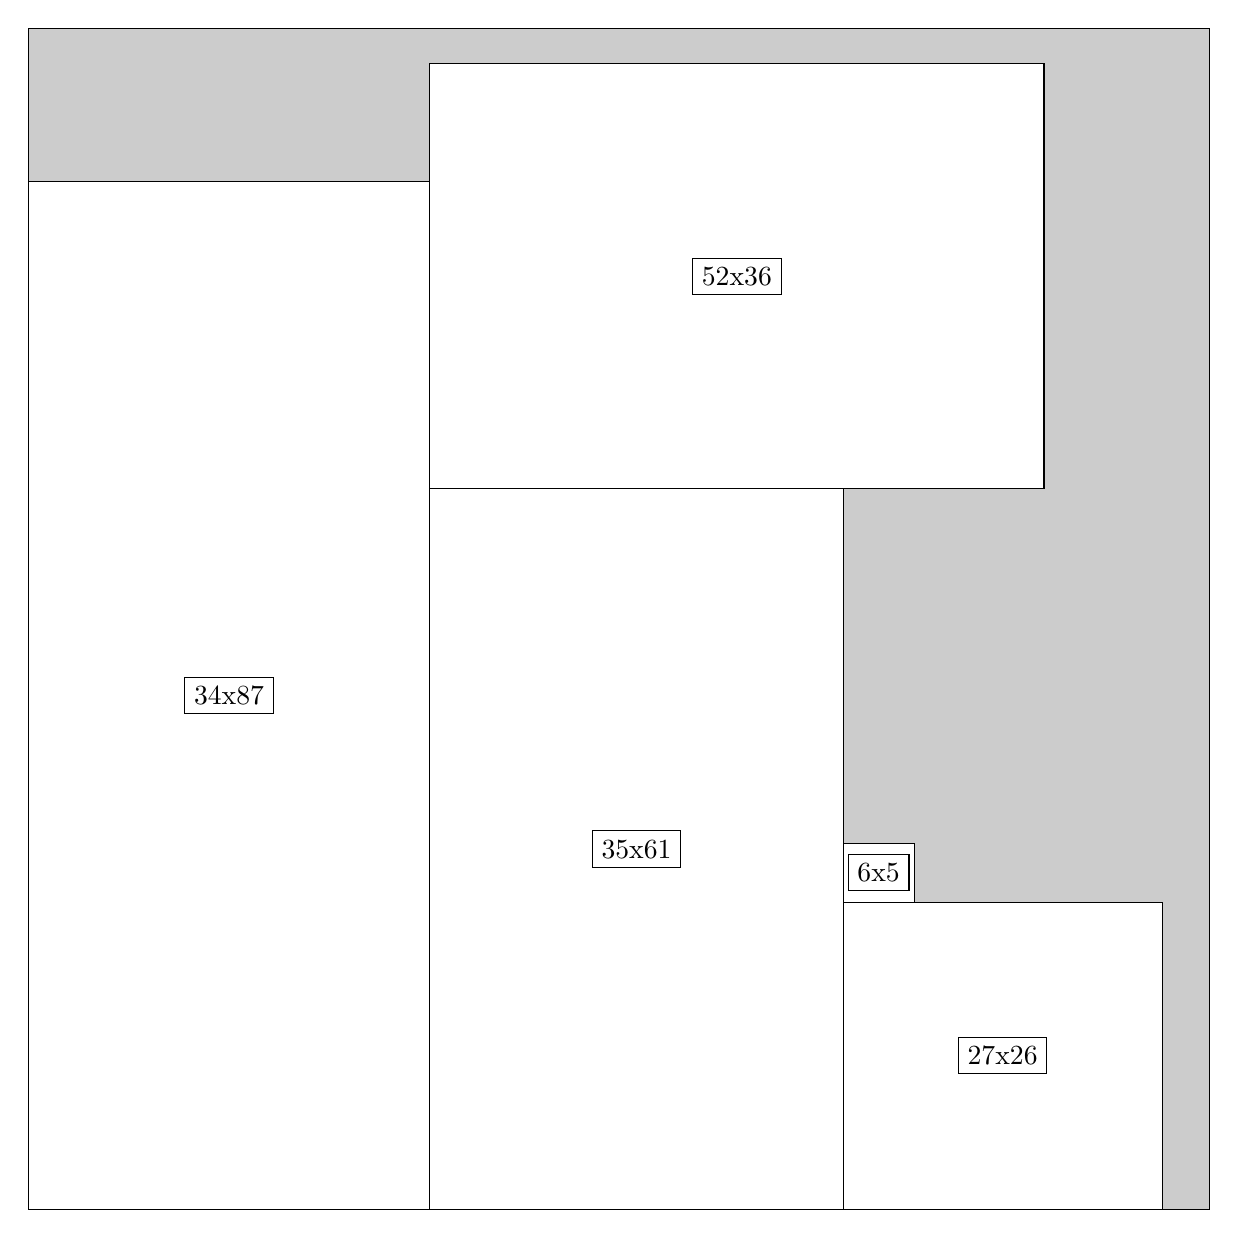
\begin{tikzpicture}[shorten >=1pt,scale=1.0,every node/.style={scale=1.0},->]
\tikzstyle{vertex}=[circle,fill=black!25,minimum size=14pt,inner sep=0pt]
\filldraw[fill=gray!40!white, draw=black] (0,0) rectangle (15.0,15.0);
\foreach \name/\x/\y/\w/\h in {34x87/0.0/0.0/5.1/13.049999999999999,35x61/5.1/0.0/5.25/9.15,52x36/5.1/9.15/7.8/5.3999999999999995,27x26/10.35/0.0/4.05/3.9,6x5/10.35/3.9/0.8999999999999999/0.75}
\filldraw[fill=white!40!white, draw=black] (\x,\y) rectangle node[draw] (\name) {\name} ++(\w,\h);
\end{tikzpicture}


w =34 , h =87 , x =0 , y =0 , v =2958
\par
w =35 , h =61 , x =34 , y =0 , v =2135
\par
w =52 , h =36 , x =34 , y =61 , v =1872
\par
w =27 , h =26 , x =69 , y =0 , v =702
\par
w =6 , h =5 , x =69 , y =26 , v =30
\par
\newpage


\end{document}